\section{Performance Evaluation}
The extension's performance goals are to provide our security guarantees without being a detriment to the end user's browsing experience. To this end, we take several timestamps throughout our code's execution. These were recorded using the Performance Web API. Note that while this API normally reports values as doubles, due to recent security threats, such as Spectre \cite{DBLP:journals/corr/abs-1801-01203}, several browser developers have implemented countermeasures by reducing the precision of the DOMHighResTimeStamp resolution \cite{reducetimeprecision,resolutionconsiderations}. In particular, Firefox reports these values as integer milliseconds. For our tests, we re-enabled higher precision values.

While our extension's functionality only applies at the network level, there is potential slowdown at the DOM processing level due to the optimization techniques the browser applies throughout several levels of the web page load pipeline. Figure ~\ref{fig:navigationtiming} presents shows the different timestamps provided by the Navigation Timing API, as well as a high-level description of the browser processing model. Since our filter listens on the onBeforeRequest event, none of the previous steps before Request are affected. In this section, we refer to the difference in time between responseEnd and requestStart as the "network filter time".

\begin{figure*}[h]
 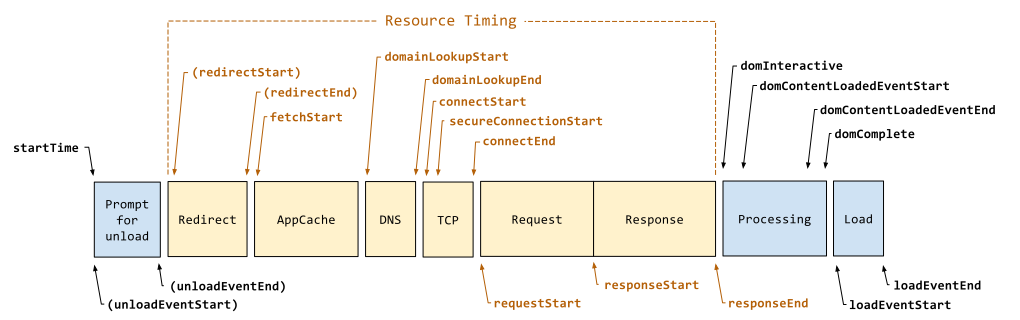
\includegraphics[scale=0.7]{img/timestamp-diagram}
 \caption{The Navigation Timing API's timestamps}
 \label{fig:navigationtiming}
 \end{figure*}

\subsection{Top websites load times}
We first report our extension's impact on top website load times, representing the expected behaviour of an user's average web browsing experience. For these tests, we first took the top 500 websites as reported by Moz.com \cite{top500}. For each website, we loaded it 25 times (with a 25 second timeout) and recorded the following values: requestStart, responseStart, responseEnd, domContentLoadedEventEnd, domComplete, duration, and decodedBodySize. From the initial 500, we only report values for 441 of them. The other 59 had consistent issues with timeouts, insecure certificates, and network errors. For our setup, we used a headless version of Firefox 6.90, and Selenium WebDriver for NodeJS, with GeckoDriver (TODO: get maas machine specs). We ran four test suites:
\begin{itemize}
	\item No extension cold cache: Firefox is loaded without the extension installed and the web driver is re-instantiated for every page load.
	\item Extension cold cache: Firefox is loaded with the extension installed and the web driver is re-instantiated for every page load.
	\item No extension warm cache: Firefox is loaded without the extension installed and the same web driver is used for the page's 25 loads.
	\item Extension warm cache: Firefox is loaded with the extension installed and the same web driver is used for the page's 25 loads.
\end{itemize}

For each set of tests, we reduced the recorded values to two comparisons: network filter (responseEnd - requestStart), and page ready (domComplete - responseStart). The first analyzes the time spent by the network filter, while the second determines the time spent until the whole document has loaded. We calculate the medians of each website for each of the previous and the decodedByteSize.

\begin{figure}[h]
	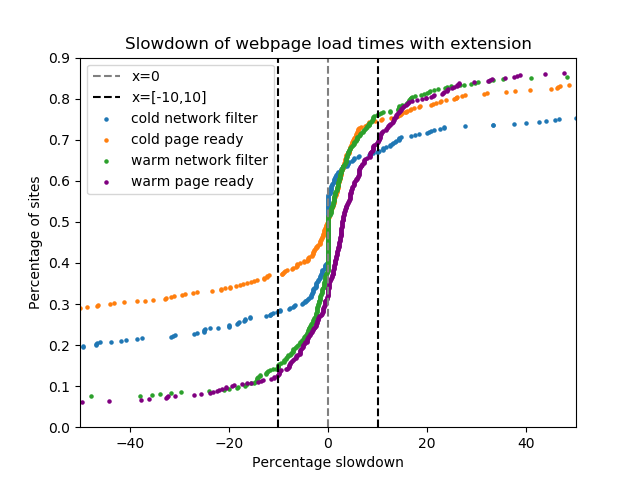
\includegraphics[scale=0.5]{results/extension_slowdown_overall}
	\caption{Cumulative distribution of relative percentage slowdown with extension installed for top sites}
	\label{fig:overall_slowdown}
\end{figure}

We compare the load times with and without the extension running by calculating the relative slowdown with the extension installed according to the following formula: 

\begin{equation*}
100*\frac{\tilde{x}_{with}-\tilde{x}_{without}}{\tilde{x}_{without}}
\end{equation*}
\\
where $\tilde{x}$ is the median with/without the extension running.

Figure ~\ref{fig:overall_slowdown} shows the computed results. We have zoomed in on the $[-50\%,50\%]$ range, as this is where the grand majority of values lie. The graph shows a slowdown of less than 10\% for 72.6\% of sites, and less than 50\% for 82\% of sites when the extension is running. Note that these values are recorded as percentages, and while some are as high as 50\%, the absolute values are in the order of seconds, and in many cases tens or hundreds of milliseconds, especially for the network component. Such values should not alter the user's experience significantly. The slowdown increases by at most 5\% when we take caching into account. We expect this to be the case because the network filter probably causes the browser to use less caching, especially for the DOM component, as it might have to process it from scratch every time.

\begin{figure}[h]
	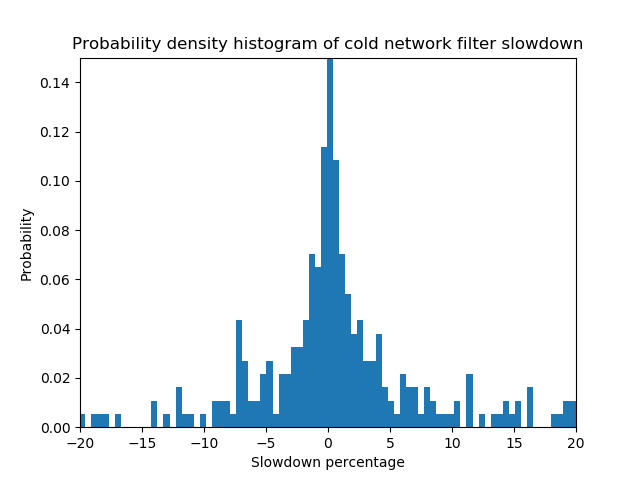
\includegraphics[scale=0.5]{results/density_histogram_filter_slowdown}
	\caption{Density histogram of network filter slowdown for top sites}
	\label{fig:histogram_slowdown}
\end{figure}


Figure ~\ref{fig:histogram_slowdown} shows a closer look at the distribution for the cold network filter slowdown on the top sites (same values as in Figure ~\ref{fig:overall_slowdown}. We filtered out any values above |100|\%, as these were mostly due to timeouts and other network delays or errors. For this component, 87.6\% of the slowdown values are less than 10\%.

\begin{figure}[h]
	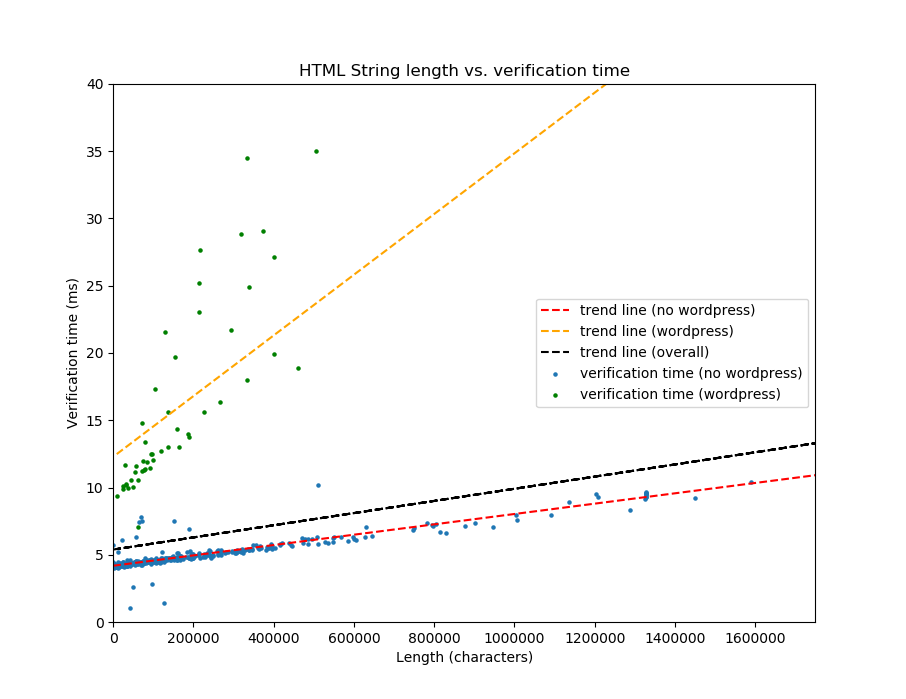
\includegraphics[scale=0.37]{results/string_length_vs_verification_time}
	\caption{Scatter plot of network filter time as a function of decoded byte size for top sites}
	\label{fig:verification_time_string_length}
\end{figure}

 Figure ~\ref{fig:verification_time_string_length} shows the time spent by the call to our string verification function in the network filter as a function of the length of the string to be verified. We loaded the same websites 25 times each and calculated the median times and lengths.  The blue dots are the pages for which the WordPress probes tested negative, and the green dots are the pages for which the probes tested positive: 55 in total (our implementation currently only has probes for WordPress). We applied least squares regression to calculate the shown trend lines. The Spearman's rank correlation values for no WordPress, WordPress, and overall are 0.910, 0.91, and 0.72 respectively, demonstrating positive correlation. Since both our probes and signatures use regex matching, we expect both trend lines to be linear, as seen in the graph. Recall that once a probe for a certain software passes, we perform a linear scan over the signatures for that specific software and check whether it applies to the given HTML string or not. Thus, we expect the slope of the line to be higher when the WordPress probe passes. Since only around 25\% of sites use WordPress on average \cite{w3techs}, we expect the impact of our network filter to be closer to the non-WordPress values, as corroborated by our overall trend line.

\begin{figure}[h]
	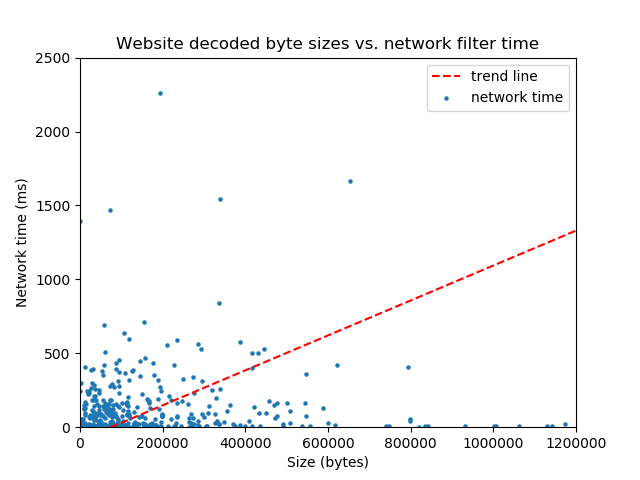
\includegraphics[scale=0.5]{results/byte_size_vs_filter_time}
	\caption{Scatter plot of network filter time as a function of decoded byte size for top sites}
	\label{fig:network_filter_decoded_size}
\end{figure}

When factoring in the rest of the network component, additional noise is introduced in the measurements. Figure ~\ref{fig:network_filter_decoded_size} shows the network filter time as a function of the page's decoded byte size. Applying least squares regression shows an upwards trend. However, the Spearman's rank correlation for this set of data is $-0.054$; we believe this to be due to the number of factors affecting this measurement. The data demonstrates that the size of the page being processed has a smaller impact than expected (see Figure ~\ref{fig:verification_time_string_length}) on the network filter time when the whole page load process is accounted for.

Additionally, for each website we recorded the number of loaded signatures (i.e. signatures whose endpoints were found in the HTML). We report a 0\% false positive rate for loaded signatures. Thus, we can infer with confidence that the rate of false positives for loaded signatures during an average user's web browsing is similarly low. This rate could possibly go up as the number of signatures and covered frameworks increases. While we can not be sure that any of the sites is free of vulnerabilities described in our current signatures, this is very unlikely, as many of these websites are not running WordPress to begin with, and being some of the most popular, they would likely be updated relatively quickly if any vulnerability is found; thus, the rate of false negatives is likely extremely low as well.

\subsection{Wordpress websites load times}

We ran similar experiments as in Section 6.1, but with the WordPress sites described in Section 4.1. Thus, all of these have either one or multiple injection points in their HTML, and the network filter will spend an additional amount of time sanitizing these as defined by the signatures. Note that the data set is smaller here, and some of the trends might be harder to infer. 

As before, Figure ~\ref{fig:wordpress_slowdown} shows the results for slowdown with the extension running. Recall that the only difference between a page which passes the WordPress probe and one that matches a signature is that the latter has to replace a portion of the original string by its sanitized version. This procedure is usually very fast, and can be faster depending on the method defined by the signature. Since even some of the top 500 sites ran WordPress, we expect a minimal difference between the two data sets. In this case we see a slowdown of less than 10\% for 88.75\% of sites, and less than 40\% for 98.75\% of them. The warm curves suffer from a smaller slowdown than the cold ones. We believe this to be the case because of the very small load times when caching is taken into account due to these pages being locally hosted, thus even minor changes in load times result in higher absolute slowdowns.

\begin{figure}[h]
	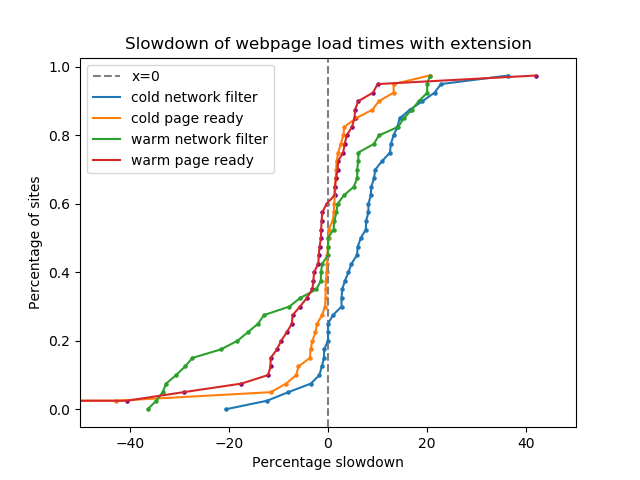
\includegraphics[scale=0.5]{results/extension_slowdown_wordpress}
	\caption{Cumulative distribution of relative percentage slowdown with extension installed for WordPress sites}
	\label{fig:wordpress_slowdown}
\end{figure}

Figure ~\ref{fig:histogram_slowdown_wordpress} shows the probability density of the cold network filter slowdown. In this case, we see that the distribution is skewed more towards a higher slowdown. As it is harder to discern the trend for this data set than its top site counterpart, we have also plotted the normal distribution of the data between 3 standard deviations. 65\% of values are less than 10\%.

\begin{figure}[h]
	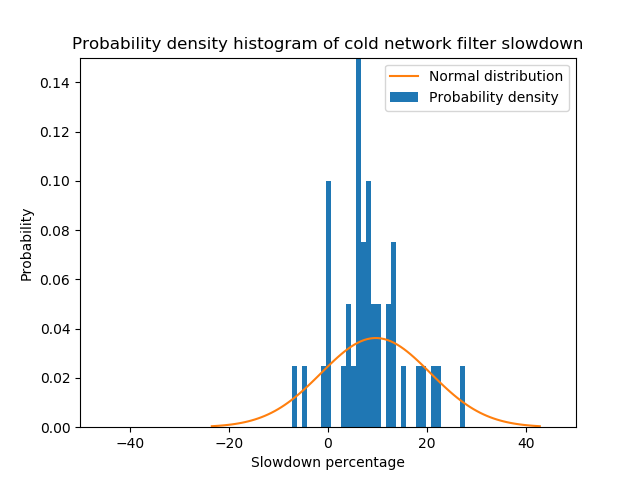
\includegraphics[scale=0.5]{results/density_histogram_filter_slowdown_wordpress}
	\caption{Density histogram of network filter slowdown for top sites}
	\label{fig:histogram_slowdown_wordpress}
\end{figure}

Finally, as in Figure ~\ref{fig:verification_time_string_length}, we report the string verification time as a function of its length, for the WordPress sites, shown in Figure ~\ref{fig:verification_time_string_length_wordpress}. The Spearman's rank correlation for this set of data is 0.630. 

\begin{figure}[h]
	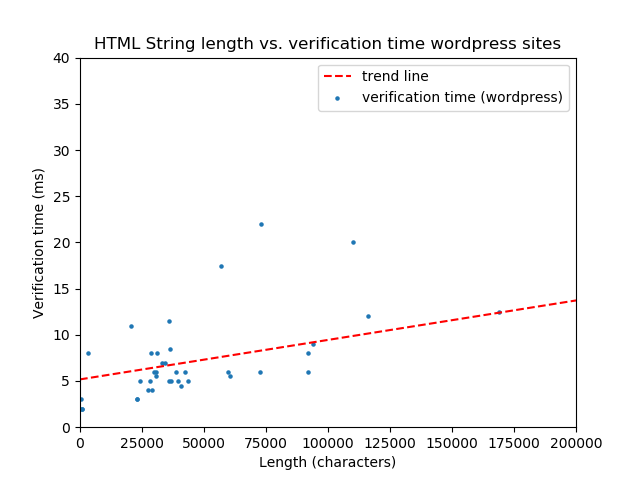
\includegraphics[scale=0.5]{results/string_length_vs_verification_time_wordpress}
	\caption{Scatter plot of network filter time as a function of decoded byte size for top sites}
	\label{fig:verification_time_string_length_wordpress}
\end{figure}